\documentclass[]{scrartcl}
\usepackage{amsmath,amssymb}
\usepackage{graphicx,xcolor}
\usepackage{algorithm}
\usepackage{hyperref}
\usepackage{listings}
\usepackage[framed,numbered]{include/mcode}

%opening
\title{ALADINp  Manual}
\author{Alexander Engelmann}




\newcommand{\Ae}[1]{\color{blue} #1\color{black}}

\begin{document}


\maketitle

\begin{abstract}

\end{abstract}

\tableofcontents

\section{Introduction}
The algorithm is based on the paper \cite{Houska}.
Few algorithmic extensions for numerical stability, e.g. a specific implementation for choosing the Hessian approximation.
Furthermore, slightly different problem formulation for numerical reasons.
We only consider the local version of ALADIN here, a globally convergent version is topic. \textcolor{red}{\textbf{TODO:} More introduction... i.e. This manual is written for ... This seems to me a bit bullett pointish..} 

\section{Problem Formulation}
The ALADIN solver solves problems of the form
\begin{subequations} \label{eq:sepForm}
	\begin{align} 
	\min_{x} \sum_{i=1}^N  f_i(x_i)& \\
	\text{subject to }\quad  g_i(x_i)&= 0 &\forall i \in \mathcal{R}, \label{sepFormEq} \\
	h_i(x_i)&\leq 0&\forall i \in \mathcal{R}, \label{sepFormInEq} \\
	\underline x_i \leq x_i& \leq \bar x_i &\forall i \in \mathcal{R}, \label{sepFormBound}\\
	\sum_{i\in \mathcal{R}} A_i x_i&=b \label{eq:consConstr},
	\end{align}
\end{subequations}
with $x=(x_1,\dots,x_N)$ and $\mathcal{R}=\{1,\dots,N\}$.
The objective functions $f_i:\mathbb{R}^{n_i}\rightarrow \mathbb{R}$, the constraint functions $g_i: \mathbb{R}^{n_{xi}} \rightarrow \mathbb{R}^{n_{gi}}$ and $h_i: \mathbb{R}^{n_{xi}} \rightarrow \mathbb{R}^{n_{hi}}$ can possibly be non-convex.
In constrast to \cite{Houska}, we distinguish here between \eqref{sepFormEq}, \eqref{sepFormInEq} and \eqref{sepFormBound} as this leads to more efficient numerical treatment.





\section{Solver Interface}
The input data for the solver are $f_i$, $g_i$, $h_i$, $A_i$, $b$, $\underline{x}_i$, $\bar x_i$, $\Sigma_i \succ 0$ and struct called opts. The objective functions $f_i$, and the constraint functions $g_i$, $h_i$ are handed over in a cell, i.e. if we have decoupled objective functions $f_1, \cdots , f_n$, they are handed over via $$
\texttt{cell\{f$_1$, f$_2$, $\cdots$, f$_n$\}}.$$
 The coupling matrices are similarly handed over via a cell, i.e. if we have $n$ coupling matrices $A_1, \cdots , A_n$ they are handed over as 
 $$\texttt{cell\{A$_1$, A$_2$ $\cdots$, A$_n$\}}.$$ Usually, every design variable has its own search domain. To transfer the feasble set to ALADIN, for each (multi dimensional) variable $x_i = (x_{i1}, \cdots , x_{in})$ a lower bound vector $\underline{x}_i = (\underline{x}_{i1}, \cdots , \underline{x}_{in})^T$ and an upper bound vector $\overline{x}_i = (\overline{x}_{i1}, \cdots , \overline{x}_{in})^T$ is transfered. All lower and upper bound vectors are again stored in two cells. $Sigma_i$ stores scaling matrices. They are handed over in the manner as the coupling matrices. The \texttt{opts} - struct contains several entries. They can be extracted from table \ref{tab: ALADIN options struct.}. \textcolor{red}{\textbf{TODO} opts struct vervollstaendigen!!!!!} 


 \Ae{Comment on default options somewhere. }
\begin{table}
	\centering
	\begin{tabular}{rcc}
		\hline
parameter & data type & typical values \\ 
\hline
$\rho^0$	& numeric  & $10^0 \dots 10^4$ \\ 
	\hline 
$r_\rho$	& numeric  & $1 \dots 2$ \\ 
	\hline 
$\rho_{\text{max}}$ & numeric & $ 5 \cdot 10^3$ \\
    \hline
$\mu^0$	& numeric  & $10^3 \dots 10^6$ \\ 
	\hline 
$r_\mu$	& numeric  & $1 \dots 2$  \\ 
	\hline 
$\mu_\text{max}$ & numeric & $10^5$ \\
    \hline
$\varepsilon$ & numeric & $10^{-4}$ \\
    \hline
\texttt{maxiter} & numeric & $15 \cdots 30$ \\
    \hline
\texttt{actMargin} & string & $-10^{-6}$ \\
    \hline
\texttt{hessian} & string & $\{\texttt{full}, \cdots \}$\\
    \hline
\texttt{solveQP}    & string  & \{\texttt{MA57, linsolve, ...} \}  \\ 
    \hline 
\texttt{reg} & string & \texttt{true}\\
    \hline
\texttt{locSol}	& string  &\{ \texttt{ipopt}, ... \} \\ 
	\hline 
\texttt{innerIter} & numeric & 2400\\
    \hline
\texttt{innerAlg} & string & \{ \texttt{full}, $\cdots$ \}\\
    \hline
\texttt{plot}	& logical  & -  \\ 
	\hline 
\texttt{Hess} & numeric & \{\texttt{standard}\} \\
    \hline
\texttt{slpGlob} & logical & - \\
    \hline
\texttt{trGamma} & numeric & $10^6$ \\    
    \hline
\texttt{Sig}	& string  & \{\texttt{Hess, const} \} \\ 
	\hline 
\texttt{term\_eps} & numeric & $10^-6$\\
    \hline
\end{tabular} 
\caption{ALADIN options struct.}
\label{tab: ALADIN options struct.}
\end{table}

\section{Software Structure}
Applying the ALADIN solver means to execute a series of different and also a series of different types of optimization problems. For the sake of readability and understanding of the software, a short recapitulation and overview of necessary general knowledge on optimization is given.

\textcolor{red}{TODO}

 An overview of the ALADIN solver in tabular form is given in figure \ref{fig:flowchart}. To be able to use the already implemented optimization tools from CasADi, first of all, the matlab functions need to be converted to CasADi functions. This is done in the function \texttt{mFun2casFun}. 
\begin{figure}[htb]
	\centering
	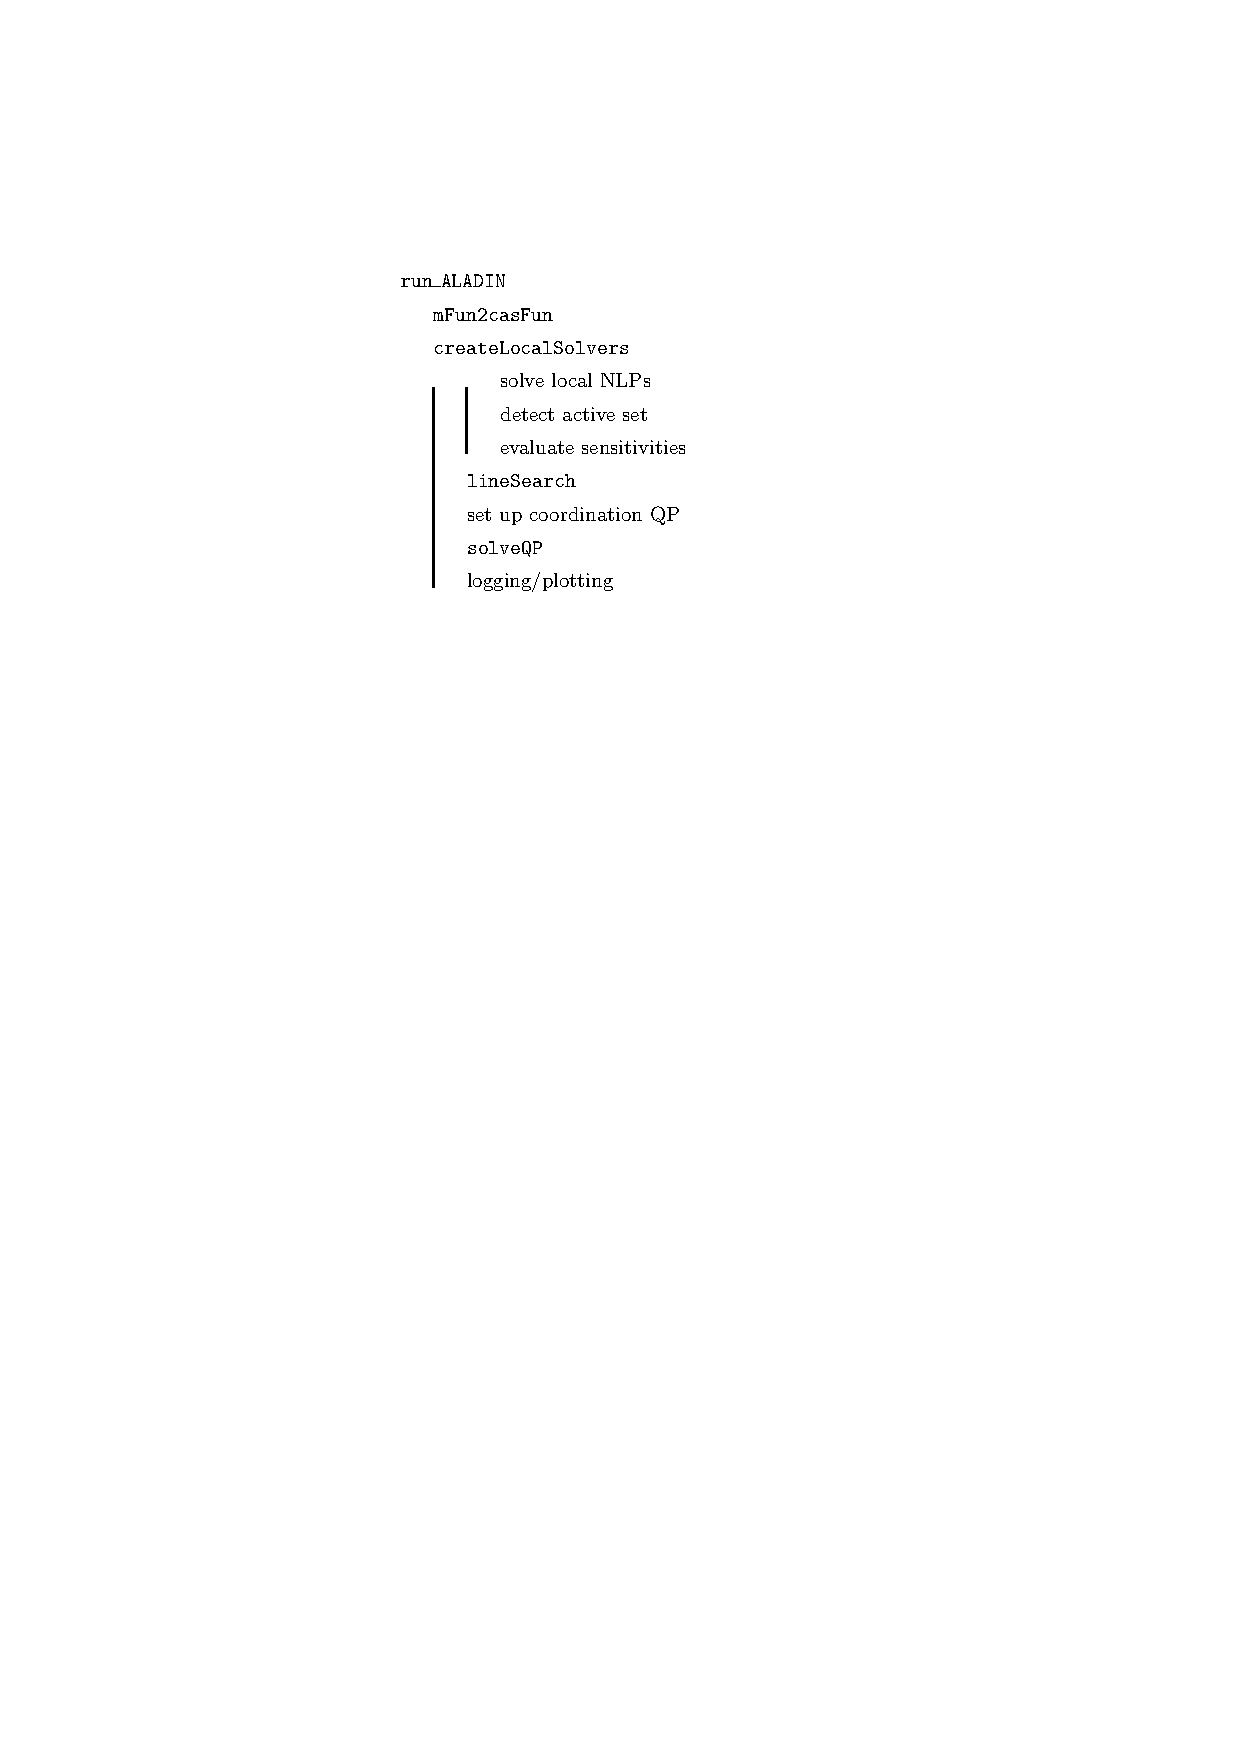
\includegraphics[width=0.3\linewidth]{figures/flowChart}
	\caption{ALADIN solver flowchart.}
	\label{fig:flowchart}
\end{figure}


\begin{algorithm}
	
	\caption{Augmented Lagrangian Alternating Direction Inexact Newto{}n (ALADIN)}
	\textbf{Initialization:} Initial guess $(z^0,\lambda^0)$, choose $\Sigma_i,\rho^0,\mu^0,\epsilon$. \\
	\textbf{Repeat:}
	\begin{enumerate}
		\item \textit{Parallelizable Step:} \label{step:parStep}
		Solve for each $i \in \mathcal{R}$
		\begin{align}
		\begin{split}
		\label{eq::denlp}
		\underset{x_i\in[\underline x_i, \overline x_i]}{\min}& f_i(x_i) + (\lambda^k)^\top A_i x_i + \hspace{-0.1em} \frac{\rho^k}{2}\left\|x_i-z_i^k\right\|_{\Sigma_i}^2
		\text{s.t.}\quad h_i(x_i) = 0 \quad \mid \kappa_i^k \quad 
		\end{split}	
		\end{align}
		\item \textit{Termination Criterion:} If 
		$
		\label{eq::stop}
		\left\|\sum_{i\in \mathcal{R}}A_ix^k_i\right\|\leq \epsilon \text{ and } \left\| x^k - z^k \right \|\leq \epsilon\;,
		$
		return $x^\star = x^k$.
		
		\item \textit{Sensitivity Evaluations:} Compute and communicate local gradients~$g_i^k=\nabla f_i(x_i^k)$,
		Hessian approximations~{$B_i^k \approx \nabla^2\{f_i(x_i^k)+\kappa_i^\top h_i(x_i^k)\}$} and constraint Jacobians $C^k_i = \nabla h_i(x^k_i)$. 
		
		\item \textit{Consensus Step:} Solve the coordination QP 
		\begin{align} 
		\notag
		&\underset{\Delta x,s}{\min}\;\;\sum_{i\in \mathcal{R}}\left\{\frac{1}{2}\Delta x_i^\top B^k_i\Delta x_i + {g_i^k}^\top \Delta x_i\right\}     + (\lambda^k)^\top s + \frac{\mu^k}{2}\|s\|^2_2  \\ 
		&\begin{aligned}\label{eq:coordQP}
		\text{s.t.}\;                                  &\quad \sum_{i\in \mathcal{R}}A_i(x^k_i+\Delta x_i) =  s     &&|\, \lambda^\mathrm{QP},\\[0.2cm]
		&\quad C^k_i \Delta x_i = 0                                    &&\forall i\in \mathcal{R},
		\end{aligned}
		\end{align}
		obtaining $\Delta x^k$ and $\lambda^{\text{QP}}$ as the solution.
		
		
		\item \textit{Line Search:} Update primal and dual variables by
		\begin{eqnarray}\notag
		z^{k+1}&\leftarrow&z^k + \alpha^k_1(x^k-z^k) + \alpha_2^k\Delta x^k \qquad \qquad
		\lambda^{k+1}\leftarrow\lambda^k + \alpha^k_3 (\lambda^\mathrm{QP}-\lambda^k),
		\end{eqnarray}
		with $\alpha^k_1,\alpha^k_2,\alpha^k_3$ from~\cite{Houska2016}. If full step 
		is accepted, i.e. $
		\alpha_1^k=\alpha_2^k=\alpha_3^k=1,
		$
		update $\rho^k$ and $\mu^k$ by
		\begin{align}
		\rho^{k+1}\;(\mu^{k+1}) =
		\begin{cases}
		r_\rho \rho^k\;(r_\mu \mu^k)   &\text{if} \; \rho^k < \bar \rho\;\; (\mu^k < \bar \mu)\\ \nonumber
		\rho^k\;(\mu^k)  &\text{otherwise} 
		\end{cases} .
		\end{align}
	\end{enumerate}
	\label{alg:ALADIN}
\end{algorithm}


\subsection{Solving the Local NLPs}
The minimum requirement for local convergence of ALADIN are local solvers and a suitable QP solver. 

\subsubsection{Active Set Detection}
We use a primal active set detection here which considers a constraint $j\in \{1,\dots,n_{hi}\}$ to be active in the current iterate if $h_{i,j}(x_i)>\epsilon_a$ where $\epsilon_a$ is a small numerical threshold (e.g. $\epsilon_a=10^{-6}$).
There are other possibilities to do so, e.g. a dual active set detection \cite{Nocedal}.
The interdependence between the active set strategy, this threshold and also the numerical solver is not fully understood yet and topic of ongoing research.
In practice it can happen, that ALADIN fails to identify the correct active set and jumps back and forth between them, cf. \autoref{sec:cycling}.

\subsubsection{Solving Local NLPs Efficiently}
In order to avoid numerical difficulties, we consider equality constraints $g$ here explicitly.
This avoids unnecessary detentions of active sets for them.

The bound constraints  \eqref{sepFormBound} are principally covered by \eqref{sepFormInEq}.
However, some solvers \cite{somePappers} can exploit their simplicity to consider them very efficiently and speeding up the local computations.


\subsection{Coordination QP}

The Lagrangian for \eqref{eq:coordQP} is
\[
L=\sum_{i\in \mathcal{R}}\left\{\textstyle \frac{1}{2}\Delta x_i^\top H^k_i\Delta x_i + {g_i^k}^\top \Delta x_i\right\} \hspace{-0.1em}  + \hspace{-0.1em} {\lambda^k}^\top  \hspace{-0.2em} s + \hspace{-0.1em}  \textstyle \frac{\mu}{2}\|s\|^2_2  + \lambda^{QP\top}(A(x^k+\Delta x)-s-b) + \kappa^{QP\top }C^{act}\Delta x.
\]
Thus, the first order optimality conditions are
\[
\nabla L =
\underbrace{
\begin{pmatrix}
H & 0 & A^\top & C^{act^\top} \\
0 &\mu I & - I & 0 \\
A & -I & 0 & 0 \\
C^{act}  & 0 & 0 & 0
\end{pmatrix}
}_{:=M_{KKT}}
\begin{pmatrix}
\Delta x \\ s \\ \lambda^{QP} \\ \kappa^{QP}
\end{pmatrix}
-
\underbrace{
\begin{pmatrix}
-g \\ - \lambda ^k \\ -Ax^k +b \\ 0
\end{pmatrix}
}_{.=m_{KKT}}
\overset{!}{=}0.
\]
As $H\succ 0$ and $C^{act}$ and $A$ are assumed to have full rank, this QP has always a unique solution.
This QP is then solved in \texttt{solveQP} or \texttt{solveQPdec} by either direct or iterative methods.

Note that if $H\succ 0$ and $C^{act}$ has full rank, $M_{KKT}$ is invertible.
If this is not the case, special care has to be taken to ensure these conditions.


\subsection{Regularization}
We have some degree of freedom in choosing the Hessian approximations $H^k$.
In any case, we have to make sure that it is positive definite to guarantee convergence of ALADIN and to make sure that the coordination QP has a solution.
In practice it may occur that $H^k$ has negative and zero eigenvalues. 
Thus we use a certain \emph{regularization} procedure to ensure positive definiteness of $H^k$.
The method we propose here is one heuristic which worked well in practice for our tested problems.
More research is needed here to come up with more systematic procedures.

In order to detect and modify zero and negative eigenvalues, we use an eigenvalue decomposition
\[
H^k=\ V\Lambda V^\top
\]
where the rows of $V$ are the eigenvectors of $H^k$ and $\Lambda$ is a diagonal matrix with the corresponding eigenvalues of $H^k$.
By modifying the eigenvalues in $\Lambda$ yielding to $\tilde \Lambda$, we can generate an approximate Hessian $\tilde H^k = V \tilde \Lambda V^\top \succ 0$.
There are different ways of modifying $\Lambda$ in the literature.
One very common approach for the zero eigenvalues is to set them to a small number $\delta$ in the range of $10^{-4}\dots 10^{-10}$.
For the negative eigenvalues, a similar approach is often used \cite{Nocedal}.
However, this did not work well for many cases and we follow a different approach here: We ``flip'' the sign of the negative eigenvalues which leads to increasingly smaller stepsizes in the corresponding direction with increasingly negative crvature.
This approach worked very well in practice, however, we would like to emphasize that this is just a heuristic and not based on depper theoretical considerations.

\subsection{The \texttt{solveQP} Subroutine}
The \texttt{solveQP} subroutine solves equality-constrained QPs of the form 
\begin{align*}
\min_x & \frac{1}{2}x^\top Hx + g^\top x \\
\text{s.t.} \;& Ax=b.
\end{align*}
There is a variety of QP solvers which are interfaced and listed in \autopageref{tab:QPsolvers}.
For big problems, it is particularly important wether the QP solver is able to exploit sparsity. 
This is only the case for some of them.


\begin{table} 
	\centering
	\begin{tabular}{rcc}
	\hline 
	solver & algorithm & sparse? \\ 
	\hline 
\texttt{linsolve}	&  &  \\ 
	\hline 
\texttt{MA57}	&  &  \\ 
	\hline 
\texttt{backslash}	&  &  \\ 
	\hline 
\texttt{MOSEK}	&  &  \\ 
	\hline 
\texttt{quadprog}	&  &  \\ 
	\hline 
\texttt{linsol}	&  &  \\ 
\hline 
\end{tabular} 
\caption{List of QP solvers.}
 \label{tab:QPsolvers}
\end{table}

\subsection{The \texttt{solveQPdec} Subroutine}
The \texttt{solveQPdec} subroutine solves the coupling QP in a decentralized fashion. 
In order to do so, it follows the procedure described in \cite{Engelmann19}.

\subsection{Experimental Features}
\subsubsection{Line Search}
So far, ALADIN usually only comes with local convergence guarantees, at least for non-convex problems. 
The globalization routines proposed in \cite{Houska} relies on solving a centralized optimization problem, which is in general not desired (and in some cases even not possible) to compute centrally.
As a heuristic, we use the $L_1$-merit function
\[
m(x,\bar \kappa) :=
\sum_{i \in \mathcal{R}} f_i(x_i) + \bar \kappa\, \|g_i(x_i)\|_1 + \bar \kappa\, \|\max(h_i(x_i),0)\|_1
\]
which is well-known from SQP methods here.\footnote{Here the inequality constraints $h_i$ also include the bounds \eqref{sepFormBound} for simplicity.}$^,$ \footnote{Note that we neglect the consensus constraint \eqref{eq:consConstr} in $m$ as it is satisfied for any portion of $\Delta x$.}
With that, we can at least get a sufficient decrease in the coordination step.

The rationale behind merit functions for globalization is quite simple: 
During the optimization problems, one would like to get ``more optimal'' and ``more feasible'' at the same time.
These two goals can be expressed in a function by summing up the objective function value plus a factor $\bar \kappa$ times some norm of the constraint violation.
Thus, by achieving a decrease in $m$, we can at the same time get a decrease in the objective function value and the constraint violation.

From the definition of $m$ one can see, that all local minimizes of \eqref{eq:sepForm} are also local minimizers of $m$. 
However, unfortunately not all local minimizers of $m$ are necessarily minimizers of \eqref{eq:sepForm}.\footnote{See \cite{Engelmann} for a counterexample.}
Nonetheless, this merit function is the basis for many globalization routines in context of SQP and we also use it here for determining the step size in the QP step.
The underlying SQP theory says, that if we have a positive definite Hessian approximation $B_i$ and certain constraint qualifications are satisfied, then there exists an $\alpha \in (0,\;1)$ and the update rule $x^+=z + \alpha \Delta x$ such that we get a sufficient decrease in $m$ \cite{Nocedal}.
With that it is actually possible to guarantee convergence to stationary points of $m$ for SQP methods.
However, as mentioned before, this might in general not be a minimizer of \eqref{eq:sepForm}, so we only ``hope'' that this is the case.

In case of ALADIN, even thi guarantee can in general not be given for the full ALADIN step.
We can only (similar as in SQP) guarantee, that we get a sufficient decrease in the merit function in the QP step.
However, as we still have the decentralized step (and this step does not necessarily produce a decent direction), we can not apply the merit function to the full step and hence also the guarantee for convergence to a stationary point of $m$ does not hold. 
However, practice has shown that in some cases using a step size rule at least for the coordination can improve convergence.
Further research is strongly needed here. 

\textcolor{blue}{Add example improving convergence here?}

\subsubsection{Lambda Initialization}
\subsubsection{$\Sigma_i=H_i$}
\subsubsection{Nonlinear Slacks}



\section{Numerical Examples}
\subsection{Problem Setup with Different Tools}
\subsubsection{MATLAB Symbolic}
\paragraph{First Example} 
As a first example, the following non-convex problem is taken into consideration

\begin{align*}
\min_{x = (x_1, x_2)} 2\cdot (x_1 - 1)^2 + (x_2 - 2)^2 &\\
\text{s.t.} \quad-1 \leq x_1 \cdot x_2 \leq 1.5.&
\end{align*}
For the application of the ALADIN solver, firstly, a reformulation is needed. Therefore, let $y_1 := (y_{11}, y_{12})$, $y_2 := (y_{21}, y_{22})$ and define
\begin{align*}
f_1(y_1) & := 2 \cdot (y_1(1) - 1 )^2 \\
f_2(y_2) & := (y_2(2) - 2)^2.
\end{align*}
Further, set
\begin{align*}
h_1(y_1) & : = 1 - y_{11} \cdot y_{12} \\
h_2(y_2) & : = -1.5 + y_{21} \cdot y_{22}.
\end{align*}
If now the follwing equations holds true, i.e.
\begin{align}\label{coupling}
\begin{aligned}
y_{11}  &= y_{21},\\
y_{12}  &= y_{22}
\end{aligned}
\end{align}
a system of separable, coupled objective functions is given. Notice, that (\ref{coupling}) can be expressed as
\begin{align*}
&\sum_{i = 1}^2 A_i y_i = 0 \\
\text{with} \quad & A_1 := \begin{bmatrix} +1 & 0 \\ 0 & +1 \end{bmatrix} \\
\text{and} \quad  & A_2 := \begin{bmatrix} -1 & 0 \\ 0 & -1 \end{bmatrix}
\end{align*}
such that overall the form of (\ref{eq:sepForm}) is given, i.e.

\begin{subequations} \label{eq:sepForm_example}
    \begin{align} 
    \min_{y} \sum_{i=1}^2  f_i(y_i)& \\
    \text{subject to }\quad  h_i(y_i)&\leq 0&\forall i \in \mathcal{R} = \{1, 2\}, \label{sepFormInEq_example} \\
    \underline y_i \leq y_i& \leq \bar y_i &\forall i \in \mathcal{R} = \{1, 2\}, \label{sepFormBound_example}\\
    \sum_{i\in \mathcal{R}} A_i y_i&=b \label{eq:consConstr_example}
    \end{align}
\end{subequations}
For implementation in \textsc{Matlab}, the objetive functions, the constraint functions, the coupling matrices and the upper and lower boundaries are handed over via a cells. The objective functions and the constraint functions are of the type \texttt{matlab function} to be able to use the matlab intern optimization toolbox. The lower boundary is stored as a vector. In the same manner, the upper boundary is stored. The coupling matrices are stored in matrix form. Further, the \texttt{opts} struct needs to be defined. Details on \texttt{opts} can be found in section TODO.
\\So firstly, for using the MATLAB symbolic toolbox, we can define the split-up problem.
\lstinputlisting[firstline=11,lastline=33]{../../examples/example_main.m}
To solve the problem using ALADIN, we first have to convert the symbolic variables to MATLAB functions
\lstinputlisting[firstline=35,lastline=40]{../../examples/example_main.m}
Next, we set the solver options
\lstinputlisting[firstline=42,lastline=52]{../../examples/example_main.m}
Finally, we solve the problem with ALADIN
\lstinputlisting[firstline=54,lastline=78]{../../examples/example_main.m}
Fig. \ref{fig:example_main} shows the convergence property of ALADIN on the first example. It can be seen that it converges after about only 10 iterations, which is very fast.

\begin{figure}
	\centering
	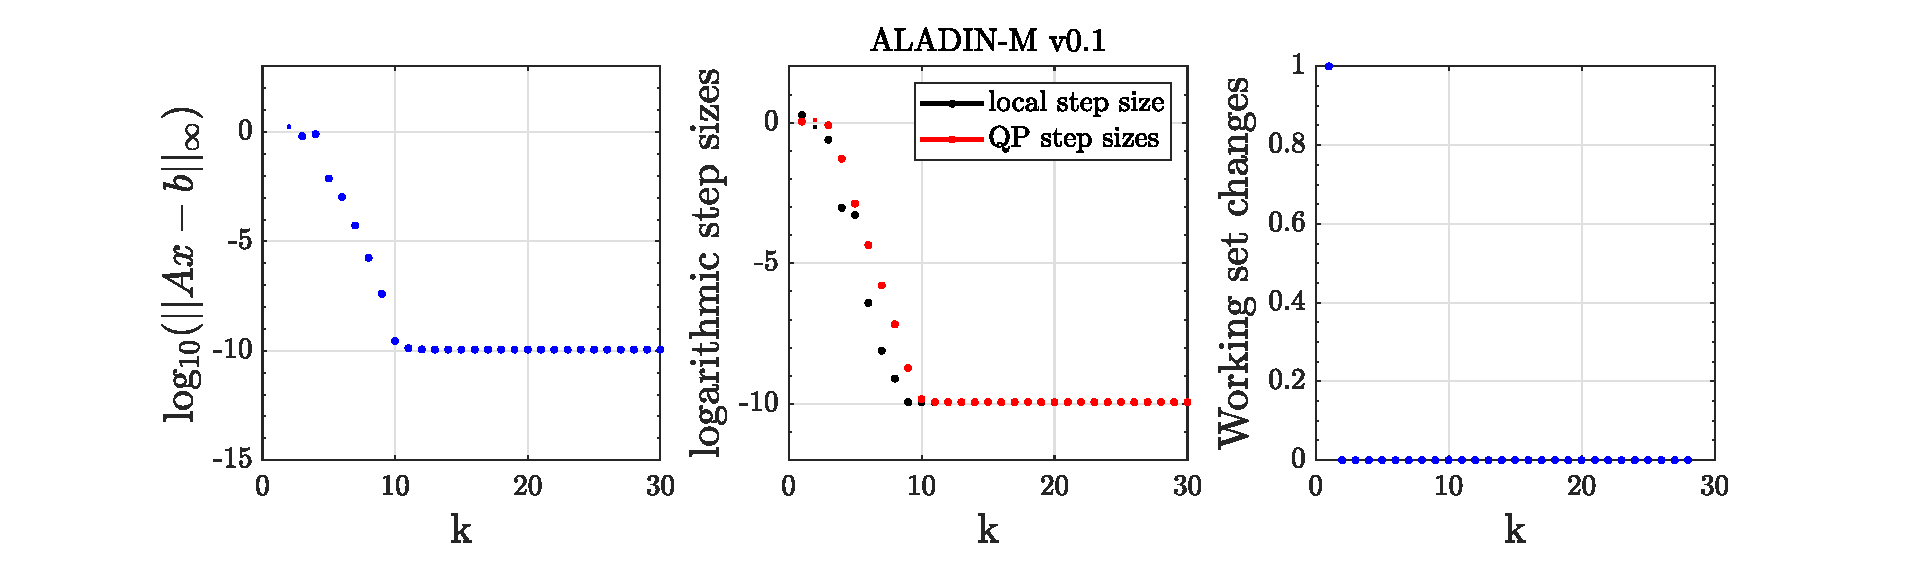
\includegraphics[width=1\linewidth]{figures/example_main.eps}
	\caption{Convergence property of ALADIN on first example}
	\label{fig:example_main}
\end{figure}

\paragraph{Rosenbrock Function} 
For the Rosenbrock Function we consider
\begin{align*}
\min_{x_1, x_2} f(x_1, x_2) &= (1 - x_1)^2 + 100 \cdot (x_2 - x_1^2)^2 \\
\text{s.t.} \quad x_1 & \geq -1.5.
\end{align*}
In order to solve it with ALADIN, we have to reformulate the problem. First, we substitute $x_1$ and $x_2$ which gives us
\begin{align*}
\min_{y_1, y_2, y_3}f(y_1, y_2, y_3) & = f(y_1) + f(y_2, y_3)\\
 & = (1 - y_1)^2 + 100 \cdot (y_3 - y_2^2)^2 \\
\text{s.t.} \quad y_2 & \geq - 1.5\\
y_1 & = y_2. 
\end{align*}
Second, we slit up the problem as follows
\begin{align*}
\min_{\tilde{y}_1, \tilde{y}_2} &= f_1(\tilde{y}_1) + f_2(\tilde{y}_2) \\
& = (1 - \tilde{y}_1)^2 + 100 \cdot (\tilde{y}_{22} - \tilde{y}_{21}^2)^2 \\ 
\\
\text{s.t.} \quad & [1] \cdot \tilde{y}_1 + [-1, 0] \cdot \tilde{y}_2 = 0 \\
\quad \quad & \quad \quad \text{ } -1.5 - \tilde{y}_{21} \leq 0
\end{align*}
with $\tilde{y}_1 = (y_1)$ and $\tilde{y}_2 = (y_2, y_3)$.
Using the MATLAB symbolic toolbox, we can now define the split-up problem 
%(see \texttt{rosenbrock\_example.m}) 
as 
\lstinputlisting[firstline=7,lastline=26]{../../examples/rosenbrock_example.m}
To solve the problem using ALADIN, we first have to convert the symbolic variables to MATLAB functions:
\lstinputlisting[firstline=28,lastline=33]{../../examples/rosenbrock_example.m}
Next, we set the solver options.
\lstinputlisting[firstline=35,lastline=40]{../../examples/rosenbrock_example.m}
Finally, we solve the problem with ALADIN
\lstinputlisting[firstline=42,lastline=56]{../../examples/rosenbrock_example.m}
Fig. \ref{fig:rosenbrock} shows the convergence property of ALADIN on Rosenbrock function.


\begin{figure}
	\centering
	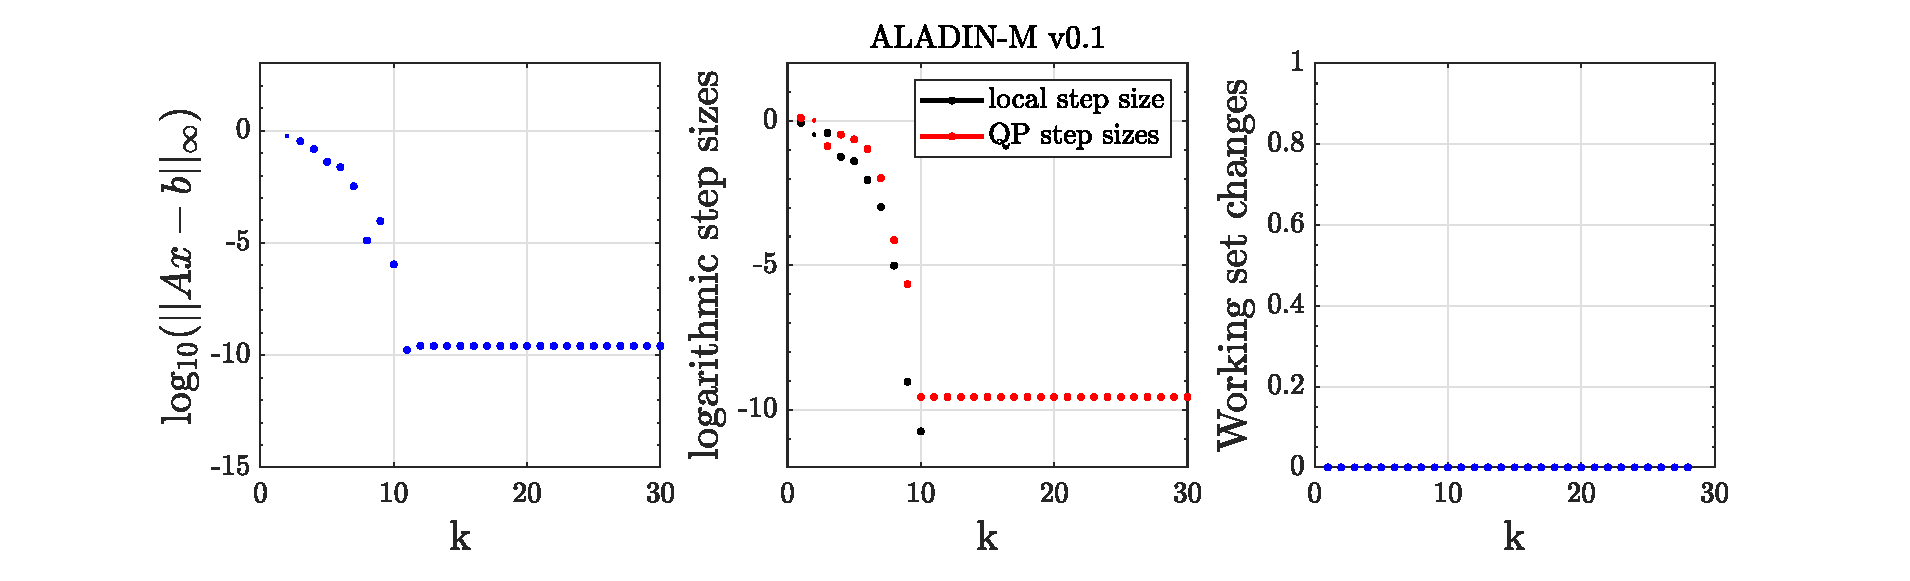
\includegraphics[width=1\linewidth]{figures/rosenbrock.eps}
	\caption{Convergence property of ALADIN on Rosenbrock function}
	\label{fig:rosenbrock}
\end{figure}

\subsubsection{MATLAB Functions}
\textcolor{red}{\textbf{TODO}} 
\subsubsection{CasADi Symbolic}
\textcolor{red}{TODO: Beispiel aufstellen für casadi symbolic statt matlab symbolic \\
$\rightarrow$ eine dependency weniger\\
$\rightarrow$ siehe \texttt{run$\_$aladin} für Beispiel.}
\subsection{Using ALADIN for MPC}
\subsection{Using ALADIN for OPF}
\subsubsection{Particular Numerical Issues in OPF}
The objective function only depends only on a very small part of the decision vector, namely on $p_g$.
Furthermore, 


\section{Known Numerical Issues}
\subsection{Cycling} \label{sec:cycling}


\appendix

\section{Additional Code}
\subsection{The \texttt{run\_ADMM} routine}
The Alternating Direction of Multipliers Method (ADMM) seems to be some kind of ``state-of-the-art'' algorithm for distributed optimization.
As it is often used as a benchmark for other algorithms and also shares some conceptual ideas with ALADIN, we included an implementation of this algorithm to the package.
We tried to make the interface of the \texttt{run\_ADMM} routine as similar as possible to the \texttt{run\_ALADIN} routine, such that the same problem setups can be used. 

We use the ADMM version of \cite{Houska} here. 






\section{Problem Reformulations}
\subsection{Consensus Reformulations in Form of \eqref{eq:sepForm}}

Problems can be reformulated in form of \eqref{eq:sepForm} quite easily.
Let us consider a ``centralized'' problem formulation
\begin{subequations} \label{eq:refProb}
	\begin{align} 
	\min_{x} \sum_{i=1}^N  f_i(x)& \\
	\text{subject to }\quad  g(x)&= 0 
	\end{align}
\end{subequations}
where we only consider equality constraints for simplicity.
Now introduce $N$ copies of $x=z_1=\dots=z_N$.
Then we can write \eqref{eq:refProb} as
\begin{align*} 
\min_{z_1,\dots,z_N} \sum_{i=1}^N  f_i(z_i)& \\
\text{subject to }\quad  g_i(z_i)&= 0, \qquad i \in \mathcal{R} \\
z_1=z_2=&\dots=z_N
\end{align*}
where the constraint functions $g_i$ are an arbitrary partitioning of $g(x)=(g_1(x),\dots,g_N(x)$ which is in form of \eqref{eq:sepForm}.
This approach is somewhat impactical as it increases the number of decision variables by a factor of $N$, 
Therefore, in practice often only a certain subset of the entries of $x$ are copied which couple the individual subsystems commonly leading to a much smaller increase of the problem size.



\end{document}
